\section{Rank-Consistency Analysis for Theorem~\ref{thm:ranking-informal}}
\label{appendix-sec:proof-thm}
This section provides a rank-consistency justification for using prompt-side entropy $V(x)$ as a low-cost proxy for response-side entropy $U^*(x)$. The result is meant to formalize the intuition behind Stage~2 under simplifying assumptions; the main empirical support for HIVE comes from the correlation and ablation results reported in the paper.

\subsection{Preliminaries and Notations}
Let the fixed model parameters be $\thetahat$ and the vocabulary size be $|\Vcal|$. We denote the sampling policy used for generation as $q(\cdot|x)$ (e.g., temperature sampling with parameter $\tau$).

\paragraph{Observable: Prompt-side Entropy.} 
Given a prompt sequence $x = (x_1, \dots, x_L)$, the model computes the probability distribution over the vocabulary at each position. Let $p_{\thetahat, \tau}(\cdot|x_{<l}) = \text{softmax}(z_{\thetahat}(x_{<l})/\tau)$ denote the temperature-scaled probability. The observable token entropy at position $l$ is $e_l(x) := \mathcal{H}(p_{\thetahat, \tau}(\cdot|x_{<l}))$. We define the aggregated prompt entropy as:
\begin{equation}
  V(x) := \frac{1}{L-1}\sum_{l=2}^{L} e_l(x).
\end{equation}
% Note that $V(x)$ is fully deterministic given the model and the prompt.

\paragraph{Observable: Response-side Entropy.} 
For a given prompt $x$, we generate $G$ independent rollouts to estimate the output entropy. For the $r$-th rollout, let the response be $y^{(r)}_{1:L_r}$. Define the step context as $c_t^{(r)} := (x, y_{<t}^{(r)})$. The token entropy at step $t$ is $u_t^{(r)}(x) := \mathcal{H}(p_{\thetahat, \tau}(\cdot|c_t^{(r)}))$. 
The length-normalized entropy for rollout $r$ is $U^{(r)}(x) := \frac{1}{L_r}\sum_{t=1}^{L_r} u_t^{(r)}(x)$.
The final empirical estimator is the average over $n$ rollouts:
\begin{equation}
  \hat{U}(x) := \frac{1}{n}\sum_{r=1}^{n} U^{(r)}(x).
\end{equation}
We define the target $U^*(x) := \mathbb{E}_{y \sim q(\cdot|x)}[U^{(r)}(x)]$ as the expected entropy under the sampling policy.

\subsection{Theoretical Bridges and Assumptions}
\label{subsec:thm-theoretical-proof}
To bridge the gap between the computationally tractable token-level logits entropy and the model's high-level semantic entropy, we establish our theoretical analysis upon two pivotal assumptions. First, we map the observable token entropy to the model's internal representation entropy (\textit{Representation Approximation}). Second, we posit that this internal entropy propagates linearly from the prompt to the response (\textit{Entropy Propagation}).

\subsubsection{From Token to Representation.}
While observable entropies $V(x)$ and $U^*(x)$ are derived from the final output layer, true epistemic entropy is often better encoded in the latent space. Following \cite{flue2025}, we define the \textit{Representation Entropy} $s(c)$ as the entropy of hidden states at a deep layer $b \approx N$, formally $s(c) \approx \hat{\mathcal{H}}[H^{(b)}|c]$. We define the aggregated representation entropies for the prompt and response as:
\begin{equation}
\begin{split}
    S_{\text{prompt}}(x) := \frac{1}{L-1}\sum_{l=2}^L s(x_{<l}),\;
    S_{\text{resp}}(x) := \mathbb{E}_{y} \left[\frac{1}{T}\sum_{t=1}^{T} s(c_t)\right].
\end{split}
\end{equation}

Based on this definition, we introduce our first assumption to link observables to internal states.

\begin{assumption}[Representation Approximation]
\label{ass:representation}
The observable token entropy approximates the internal representation entropy up to a small residual $\delta$:
\begin{equation}
  |V(x) - S_{\text{prompt}}(x)| \le \delta \quad \text{and} \quad |U^*(x) - S_{\text{resp}}(x)| \le \delta.
\end{equation}
\end{assumption}
\noindent\textit{{Justification (Theoretical):}} This assumption is grounded in Proposition 1 of \cite{flue2025}, which proves that for trained LLMs, the entropy of hidden states in deep layers serves as an approximate upper bound for the predictive posterior entropy (i.e., our token entropy). As the layer depth $b \to N$, the mutual information is maximized, ensuring the token entropy is tightly correlated with the internal representation.

% \subsubsection{Entropy Propagation.}
% Having established the link to internal representations, we next model how this entropy evolves from the input context to the generation phase.

% \begin{assumption}[Entropy Propagation]
% \label{ass:propagation}
% The representation entropy in the prompt propagates linearly to the response generation stage. There exist constants $a > 0, b \in \mathbb{R}$ such that:
% \begin{equation}
%   |S_{\text{resp}}(x) - (a S_{\text{prompt}}(x) + b)| \le \epsilon.
% \end{equation}
% \end{assumption}

% % \begin{figure}[t]
    \centering
    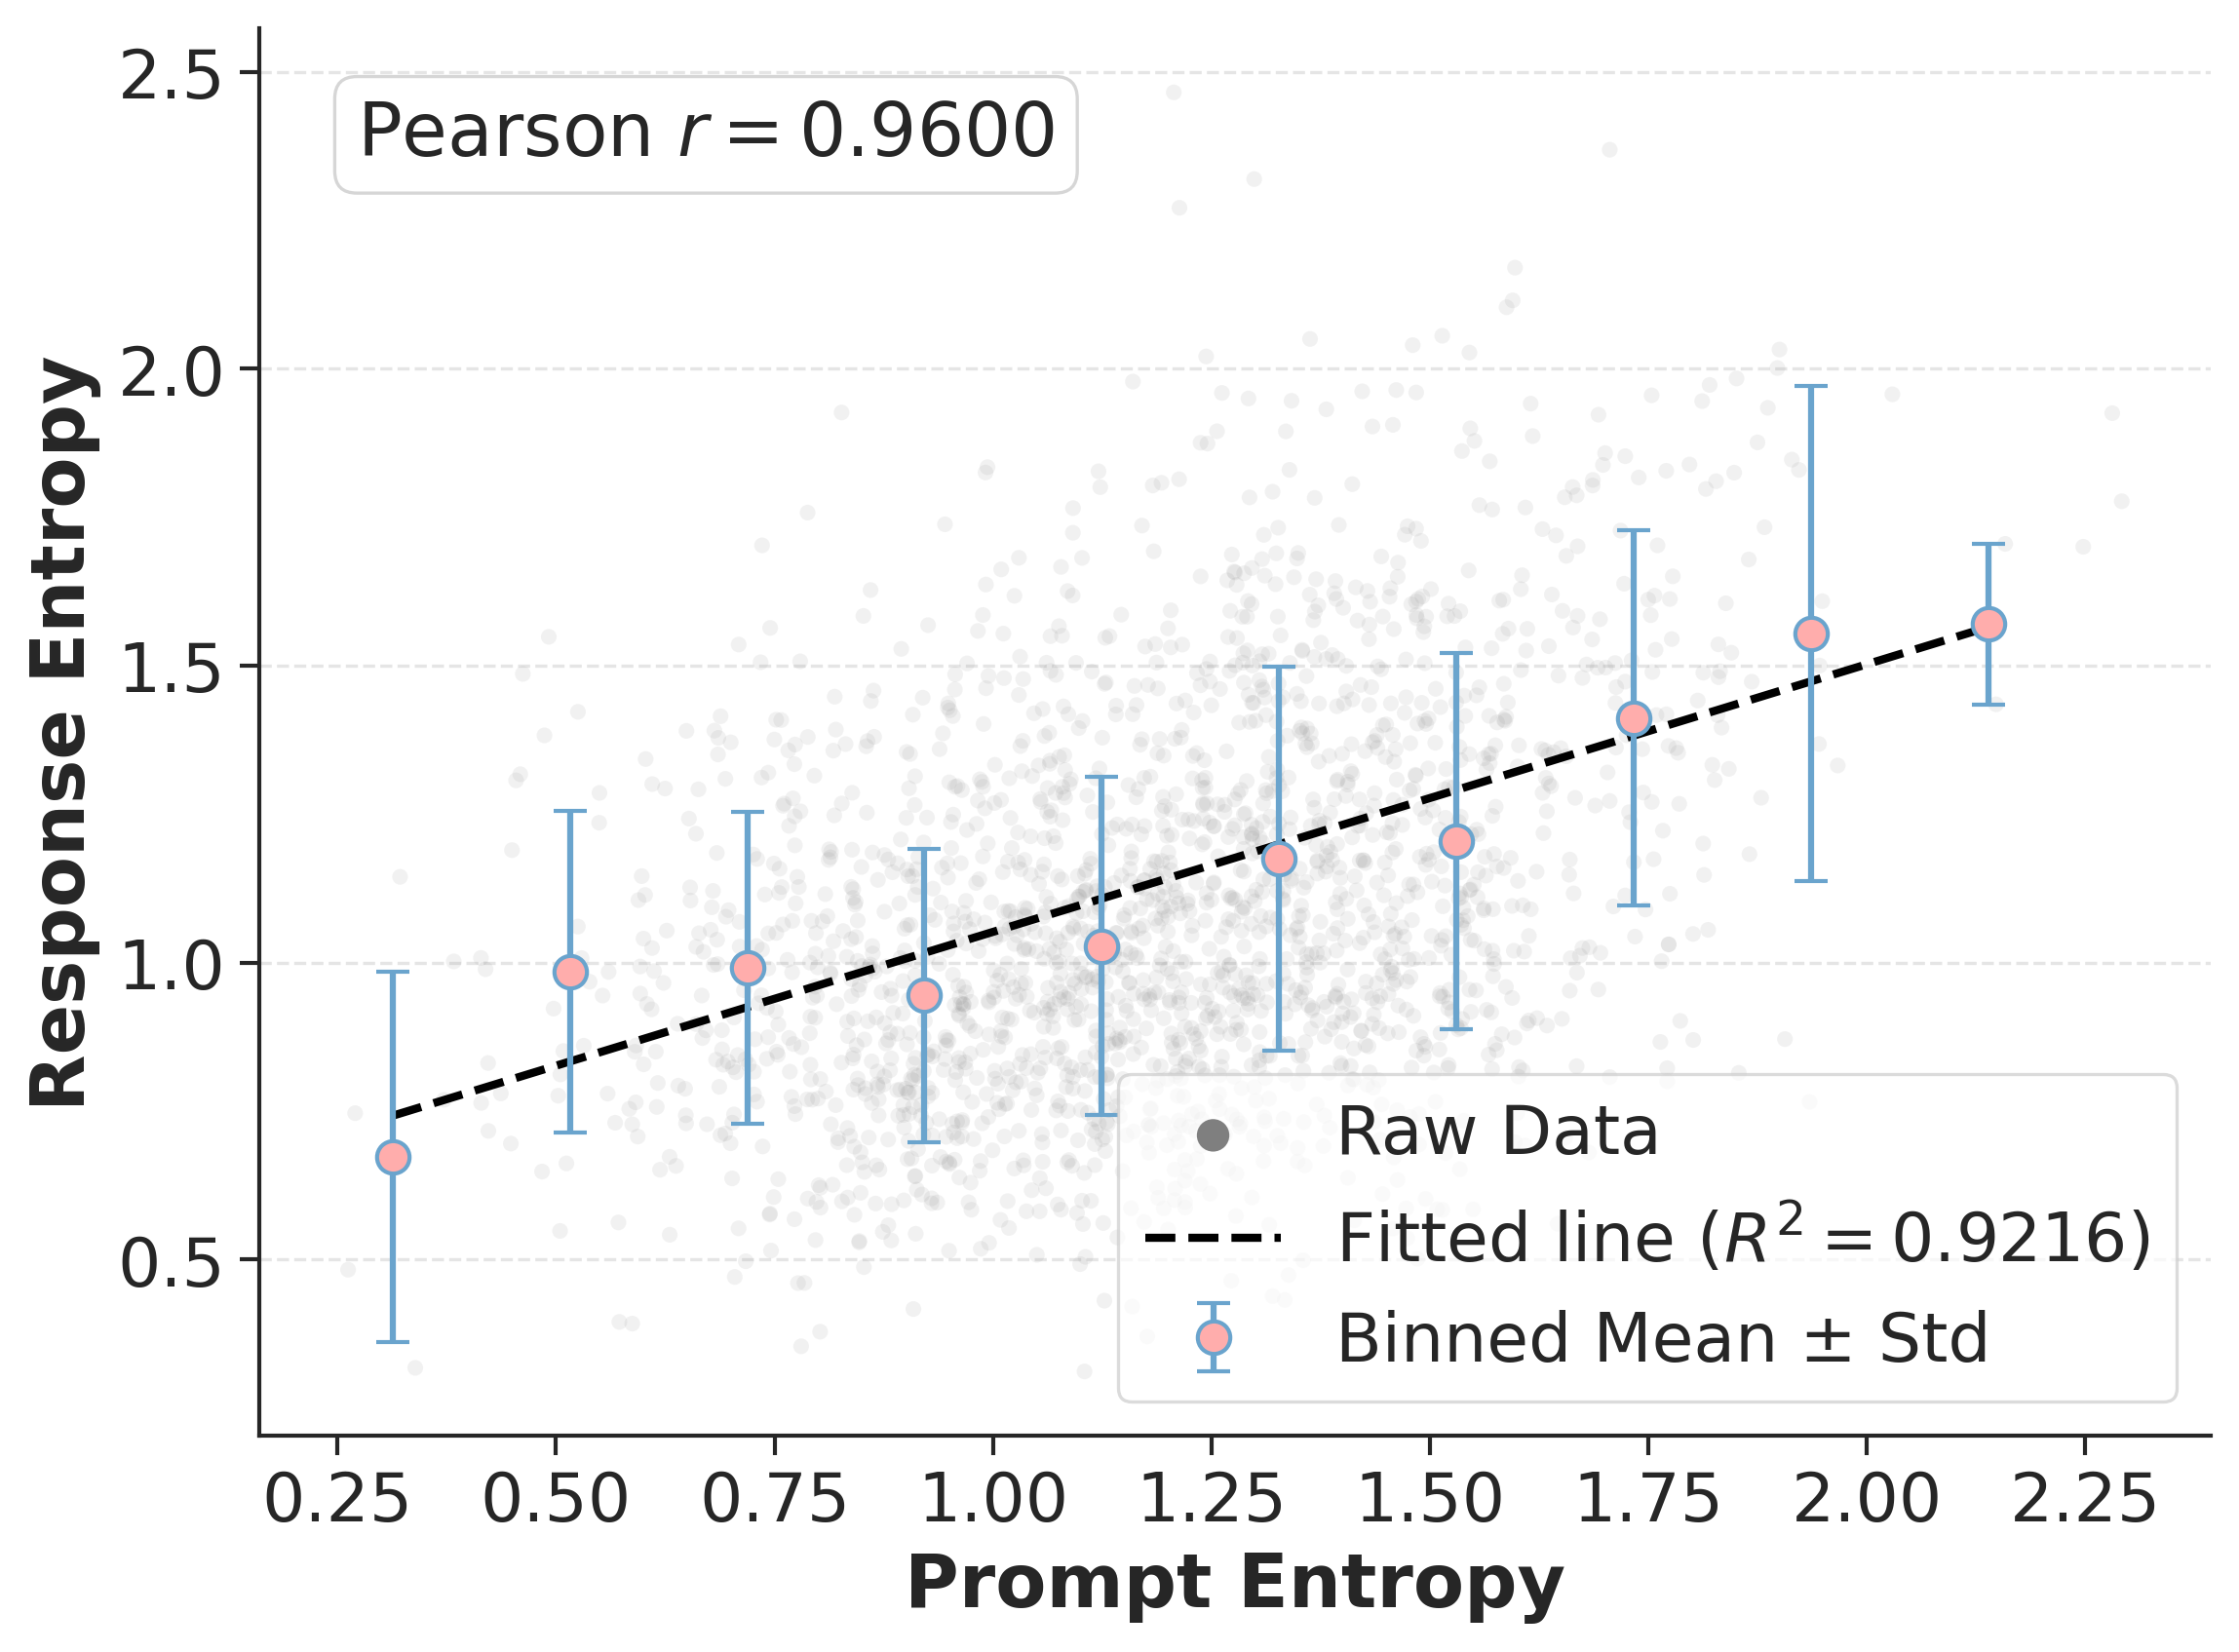
\includegraphics[width=\linewidth]{figures/appendix/binned_mean_respRatio15-beauty.png}
    \captionof{figure}{\textbf{Empirical support for entropy propagation (Assumption~\ref{ass:propagation}).} The scatter plot shows the relationship between prompt mean entropy and response entropy over 2,048 samples. We report binned statistics (blue points, mean $\pm$ std) to separate the average trend from sample-level generation noise (grey dots). The regression line on the binned data has $R^2=0.9216$ and Pearson $r=0.9600$, supporting prompt-side entropy as a response-side entropy proxy.}%By focusing on the top-tier entropy tokens, we capture the propagation of semantic uncertainty as characterized by \cite{wang2025beyond}.
    \label{fig:entropy_correlation}
    % \vspace{-3mm} % 可选：微调Caption与正文之间的距离，节省空间
% \end{figure}

\noindent % 防止首行缩进造成未对齐
\subsubsection{Entropy Propagation.}

% --- 开始 Wrapfigure 环境 ---
% {r} 表示靠右，{0.45\textwidth} 是图片区域宽度，可根据需要调整
\begin{wrapfigure}{r}{0.45\textwidth} 
    \vspace{-20pt} % 【调整核心】向上移动图片，使其与左侧标题/正文顶部对齐
    \centering
    
    % 这里插入你的图片内容
    % 注意：被 input 的文件内不能有 \begin{figure} 环境，只能有纯图片代码
    % \begin{figure}[t]
    \centering
    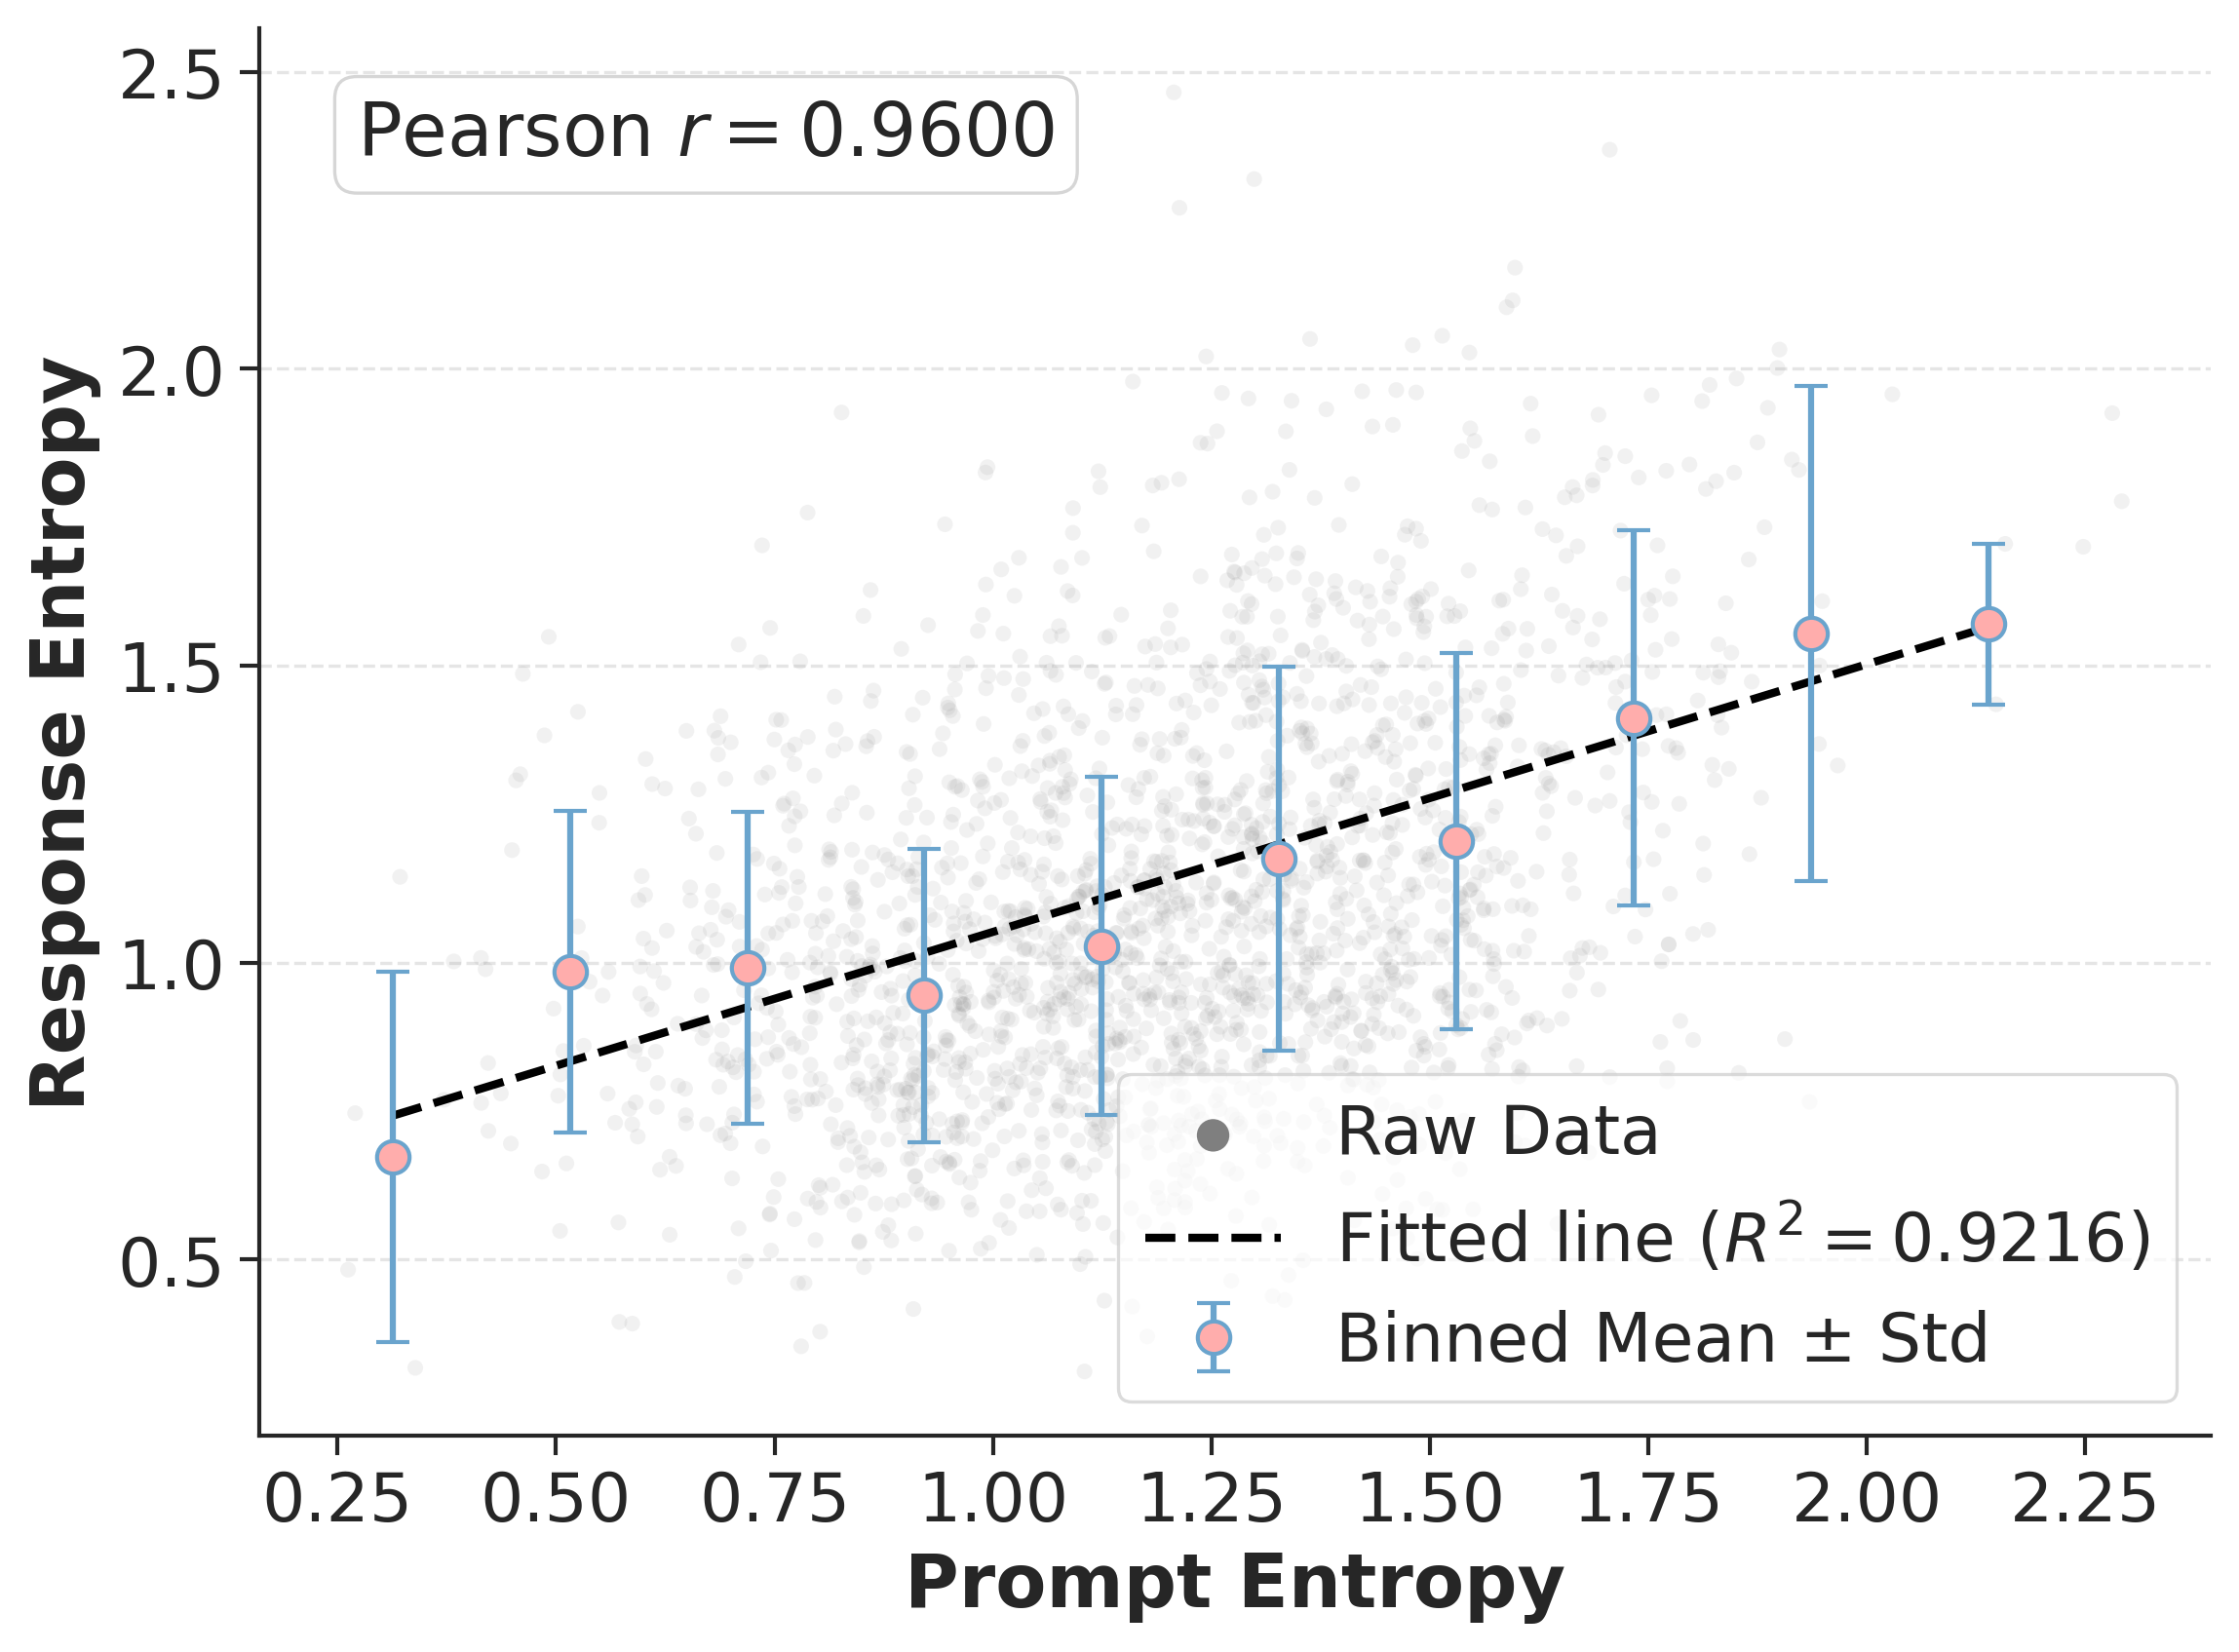
\includegraphics[width=\linewidth]{figures/appendix/binned_mean_respRatio15-beauty.png}
    \captionof{figure}{\textbf{Empirical support for entropy propagation (Assumption~\ref{ass:propagation}).} The scatter plot shows the relationship between prompt mean entropy and response entropy over 2,048 samples. We report binned statistics (blue points, mean $\pm$ std) to separate the average trend from sample-level generation noise (grey dots). The regression line on the binned data has $R^2=0.9216$ and Pearson $r=0.9600$, supporting prompt-side entropy as a response-side entropy proxy.}%By focusing on the top-tier entropy tokens, we capture the propagation of semantic uncertainty as characterized by \cite{wang2025beyond}.
    \label{fig:entropy_correlation}
    % \vspace{-3mm} % 可选：微调Caption与正文之间的距离，节省空间
% \end{figure}

    
    % 如果你的 input 文件里没有 caption，请在这里加：
    % \caption{Validation of Entropy Propagation...}
    % \label{fig:entropy_correlation}
    
    \vspace{-10pt} % 减少图片下方的空白
\end{wrapfigure}
% --- 结束 Wrapfigure 环境 ---

% 左侧的文字会自动填充在图片左边
Having established the link to internal representations, we next model how this entropy evolves from the input context to the generation phase.

\begin{assumption}[Entropy Propagation]
\label{ass:propagation}
The representation entropy in the prompt propagates linearly to the response generation stage. There exist constants $a > 0, b \in \mathbb{R}$ such that:
\begin{equation}
  |S_{\text{resp}}(x) - (a S_{\text{prompt}}(x) + b)| \le \epsilon.
\end{equation}
\end{assumption}

% 当文字长度超过图片高度时，下方的文字会自动变宽，填满图片下方的空白
\noindent\textit{{Justification (Empirical):}} To examine this linearity and quantify the noise $\epsilon$, we analyzed 2,048 prompts. We computed $V(x)$ as the proxy for $S_{\text{prompt}}$ (per Assumption~\ref{ass:representation}). %For the response side, to capture effective semantic entropy and avoid dilution by low-entropy functional tokens, we applied a \textit{High-Entropy Filtering} strategy (averaging the top 15\% entropy tokens across 8 rollouts). This strategy aligns with findings in~\cite{wang2025beyond}, who demonstrates that reasoning is driven by a ``high-entropy minority" of tokens (``forks"). 
To mitigate the intrinsic stochasticity of LLM generation, we use a binned analysis. As shown in Figure~\ref{fig:entropy_correlation}, prompt-side and response-side entropy have a strong positive correlation (Pearson $r$=0.9600). The binned mean trend is well approximated by a line with $R^2=0.9216$, supporting the linear structure in Assumption~\ref{ass:propagation} for the regimes studied here.

\subsection{Concentration Bound}
\begin{lemma}[High-probability Concentration]
\label{lemma:concentration}
For any fixed prompt $x$ and tolerance $\eta > 0$, the empirical entropy $\hat{U}(x)$ concentrates around the true expectation $U^*(x)$:
\begin{equation}
  \Pr\left(|\hat{U}(x) - U^*(x)| > \eta\right) \le 2 \exp\left( - \frac{2n\eta^2}{(\log|\Vcal|)^2} \right).
  \label{eq:concentration_prob}
\end{equation}
Consequently, for any confidence level $1-\alpha$ (where $\alpha \in (0, 1)$), with probability at least $1-\alpha$:
\begin{equation}
  |\hat{U}(x) - U^*(x)| \le \eta(\alpha) := \log|\Vcal| \sqrt{\frac{\log(2/\alpha)}{2n}}.
  \label{eq:concentration_bound}
\end{equation}
\end{lemma}

\begin{proof}
The sequence-level entropy $U^{(r)}(x)$ for each rollout is bounded within $[0, \log|\Vcal|]$. Since the $G$ rollouts are generated independent and identically distributed (i.i.d.) from the sampling policy $q(\cdot|x)$, Hoeffding's inequality~\cite{hoeffding1963probability} applies directly to the empirical mean $\hat{U}(x)$, yielding the stated bound.
\end{proof}

\subsection{Main Result: Rank Consistency}

\begin{theorem}[Theorem~\ref{thm:ranking-informal}]
\label{thm:ranking-appendix}
Consider a pair of prompts $(x, x')$. Let $\Delta_V := V(x) - V(x')$ be the observable difference in prompt entropy, and $\Delta_U := \hat{U}(x) - \hat{U}(x')$ be the difference in estimated response entropy. Under Assumptions \ref{ass:representation} and \ref{ass:propagation}, for any $\alpha \in (0, 1)$, with probability at least $1-2\alpha$:
\begin{equation}
  |\Delta_U - a\Delta_V| \le 2\epsilon + 2(a+1)\delta + 2\eta(\alpha).
  \label{eq:theorem_bound-appendix}
\end{equation}
Crucially, if the prompt entropy margin satisfies $|a\Delta_V| > 2\epsilon + 2(a+1)\delta + 2\eta(\alpha)$, then the ranking is preserved:
\begin{equation}
  \text{sign}(\hat{U}(x) - \hat{U}(x')) = \text{sign}(V(x) - V(x')).
  \label{eq:theorem_order-appendix}
\end{equation}
\end{theorem}

\begin{proof}
We decompose the error into three components: sampling noise, propagation residual, and representation approximation error.

\noindent\textbf{Step 1: Sampling Noise.} By applying Lemma \ref{lemma:concentration} and a union bound over prompts $x$ and $x'$, with probability $\ge 1-2\alpha$, the empirical estimates are close to their true expectations:
\begin{equation}
  |\Delta_U - (U^*(x) - U^*(x'))| \le 2\eta(\alpha).
  \label{eq:step1}
\end{equation}

\noindent\textbf{Step 2: Propagation Dynamics.} From Assumption \ref{ass:propagation}, we express the response representation entropy as $S_{\text{resp}}(x) = a S_{\text{prompt}}(x) + b + \xi(x)$ where $|\xi(x)| \le \epsilon$. The difference between two prompts cancels out the bias term $b$:
\begin{equation}
  |(S_{\text{resp}}(x) - S_{\text{resp}}(x')) - a(S_{\text{prompt}}(x) - S_{\text{prompt}}(x'))| \le 2\epsilon.
  \label{eq:step2}
\end{equation}

\noindent\textbf{Step 3: Representation Approximation.} Using Assumption \ref{ass:representation}, we substitute the theoretical representation entropies with observable token entropies. We have $|(U^*(x) - U^*(x')) - (S_{\text{resp}}(x) - S_{\text{resp}}(x'))| \le 2\delta$ and $|(S_{\text{prompt}}(x) - S_{\text{prompt}}(x')) - \Delta_V| \le 2\delta$. 
Applying the triangle inequality and scaling the prompt-side error by $a$:
\begin{equation}
  |(U^*(x) - U^*(x')) - a\Delta_V| \le 2\epsilon + 2\delta + 2a\delta = 2\epsilon + 2(a+1)\delta.
  \label{eq:step3}
\end{equation}

Combining Eq. \eqref{eq:step1} and Eq. \eqref{eq:step3} yields the final bound in Eq. \eqref{eq:theorem_bound-appendix}. The condition $|a\Delta_V| > \text{RHS}$ (Right-Hand Side) ensures that the signal magnitude exceeds the worst-case cumulative noise, guaranteeing that the sign of the difference remains unchanged.
\end{proof}
